% !TEX root = BachelorBookletMain.tex

\chapter{Resources}
\section{Software}
\begin{itemize}
\item Unity3D
\item Git
\item Visual Studio
\item Python
\item PyCharm
\item Blender
\item Krita
\end{itemize}

\section{Unity packages}
\begin{itemize}
\item MK Toon Free (Toon shader) % & https://assetstore.unity.com/packages/vfx/shaders/mk-toon-free-68972 \\
\item Post Processing Stack % & https://assetstore.unity.com/packages/essentials/post-processing-stack-83912 \\
\item Universal Sound FX % & https://assetstore.unity.com/packages/audio/sound-fx/universal-sound-fx-17256 \\
\item Standard Assets % & https://assetstore.unity.com/packages/essentials/asset-packs/standard-assets-32351 \\
\item Ultimate Game Music Collection % & https://assetstore.unity.com/packages/audio/music/orchestral/ultimate-game-music-collection-37351 \\
\item Resonance Audio SDK for Unity v1.2.1 % & https://github.com/resonance-audio/resonance-audio-unity-sdk/releases \\
\end{itemize}

\section{Python packages}
\begin{tabular}{| r | l || r | l |}
\hline
absl-py             & 0.6.1 &
altgraph            & 0.16.1 \\
astor               & 0.7.1 &
certifi             & 2018.10.15 \\
Click               & 7.0 &
cycler              & 0.10.0 \\
Cython              & 0.29 &
dist-keras          & 0.2.1 \\
Flask               & 1.0.2 &
future              & 0.17.1 \\
gast                & 0.2.0 &
grpcio              & 1.12.1 \\
h5py                & 2.8.0 &
itsdangerous        & 1.1.0 \\
Jinja2              & 2.10 &
Keras               & 2.2.4 \\
Keras-Applications  & 1.0.6 &
Keras-Preprocessing & 1.0.5 \\
keyboard            & 0.13.2 &
kiwisolver          & 1.0.1 \\
macholib            & 1.11 &
Markdown            & 3.0.1 \\
MarkupSafe          & 1.0 &
matplotlib          & 3.0.1 \\
mkl-fft             & 1.0.6 &
mkl-random          & 1.0.1 \\
names               & 0.3.0 &
numpy               & 1.15.3 \\
olefile             & 0.46 &
pandas              & 0.23.4 \\
pefile              & 2018.8.8 &
Pillow              & 5.3.0 \\
pip                 & 10.0.1 &
protobuf            & 3.6.1 \\
pygame              & 1.9.4 &
PyInstaller         & 3.4 \\
pyparsing           & 2.2.2 &
PyQt5               & 5.11.2 \\
PyQt5-sip           & 4.19.12 &
python-dateutil     & 2.7.5 \\
pytz                & 2018.7 &
pywin32-ctypes      & 0.2.0 \\
PyYAML              & 3.13 &
scipy               & 1.1.0 \\
setuptools          & 39.1.0 &
six                 & 1.11.0 \\
tensorboard         & 1.11.0 &
tensorflow          & 1.11.0 \\
termcolor           & 1.1.0 &
Theano              & 1.0.3 \\
tornado             & 5.1.1 &
Werkzeug            & 0.14.1 \\
wheel               & 0.32.2 &
wincertstore        & 0.2 \\
\hline
\end{tabular}
\newpage

\section{Textures}
\begin{centering}
\begin{tabular}{l|l}
Texture & Source \\
\hline

\includegraphics[width=0.2\textwidth]{Images/textures/BlackBorder.png} &  \\

\includegraphics[width=0.2\textwidth]{Images/textures/BlackThickBorder.png} &
\makecell[l]{Given on the 8.12.2018 \\ by Yannick Pawils} \\
\hline
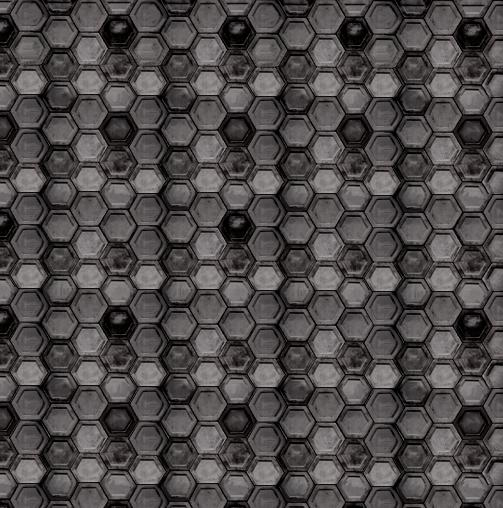
\includegraphics[width=0.2\textwidth]{Images/textures/airbase_radar_panels.jpg} &
\makecell[l]{Retrieved on the 8.12.2018 from \\ \linebreak https://opengameart.org/node/7254}
\end{tabular}
\end{centering}
